\documentclass[11pt]{standalone}

\usepackage{helvet}
\usepackage{units}
\usepackage{textcomp}

\usepackage{ifthen}
\usepackage{tikz} 
\usetikzlibrary{shapes.misc}
\usetikzlibrary{arrows,arrows.meta}
\usetikzlibrary{calc,intersections, patterns, math}
\usetikzlibrary{decorations.pathmorphing}
\usetikzlibrary{shapes.geometric}

\definecolor{pfeil}{RGB}{168,167,167}
\definecolor{petrol}{RGB}{0, 118, 136}
\definecolor{blue}{RGB}{0, 118, 136}
% \definecolor{blue}{RGB}{100, 100, 255}
\definecolor{darkgoldenrod}{RGB}{184, 134, 11}
\colorlet{petrol-lighter}{petrol!40}
\colorlet{darkgoldenrod-lighter}{darkgoldenrod!40}

\begin{document}

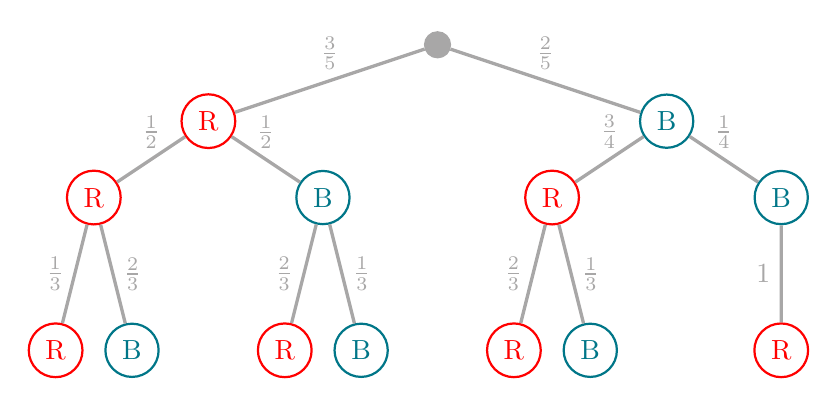
\begin{tikzpicture}[pfeil,yscale=-1,scale=0.97, xscale=-1]
	\node[draw,fill,circle] (S) at (0,0) {};
		\node[draw,circle, thick, red] (K1) at (3,1) {R};
		\node[draw,circle, thick, blue] (Z1) at (-3,1) {B};
		\draw[very thick] (S) -- node[above] {$\frac 35$} (K1);
		\draw[very thick] (S) -- node[above] {$\frac 25$} (Z1);
		\node[draw,circle, thick, red] (K21) at (4.5,2) {R};
		\node[draw,circle, thick, blue] (Z21) at (1.5,2) {B};
		\draw[very thick] (K1) -- node[above] {$\frac 12$} (K21);
		\draw[very thick] (K1) -- node[above] {$\frac 12$} (Z21);
		\node[draw,circle, thick, red] (K22) at (-1.5,2) {R};
		\node[draw,circle, thick, blue] (Z22) at (-4.5,2) {B};
		\draw[very thick] (Z1) -- node[above] {$\frac 34$} (K22);
		\draw[very thick] (Z1) -- node[above] {$\frac 14$} (Z22);
		\node[draw,circle, thick, red] (K31) at (5,4) {R};
		\node[draw,circle, thick, blue] (Z31) at (4,4) {B};
		\draw[very thick] (K21) -- node[left] {$\frac 13$} (K31);
		\draw[very thick] (K21) -- node[right] {$\frac 23$} (Z31);
		\node[draw,circle, thick, red] (K32) at (2,4) {R};
		\node[draw,circle, thick, blue] (Z32) at (1,4) {B};
		\draw[very thick] (Z21) -- node[left] {$\frac 23$} (K32);
		\draw[very thick] (Z21) -- node[right] {$\frac 13$} (Z32);
		
		\node[draw,circle, thick, red] (K33) at (-1,4) {R};
		\node[draw,circle, thick, blue] (Z33) at (-2,4) {B};
		\draw[very thick] (K22) -- node[left] {$\frac 23$} (K33);
		\draw[very thick] (K22) -- node[right] {$\frac 13$} (Z33);
		\node[draw,circle, thick, red] (K34) at (-4.5,4) {R};
		\draw[very thick] (Z22) -- node[left] {$1$} (K34);
   

    




\end{tikzpicture}




\end{document}
